%%%%%%%%%%%%%%%%%%%%%%%%%%%%%%%%%%%%%%%%%%%%%%%%%%%%%%%%%%%%%%%%%%%%%
%% This is a (brief) model paper using the achemso class
%% The document class accepts keyval options, which should include
%% the target journal and optionally the manuscript type. 
%%%%%%%%%%%%%%%%%%%%%%%%%%%%%%%%%%%%%%%%%%%%%%%%%%%%%%%%%%%%%%%%%%%%%
\documentclass[journal=jacsat,manuscript=article]{achemso}

%%%%%%%%%%%%%%%%%%%%%%%%%%%%%%%%%%%%%%%%%%%%%%%%%%%%%%%%%%%%%%%%%%%%%
%% Place any additional packages needed here.  Only include packages
%% which are essential, to avoid problems later. Do NOT use any
%% packages which require e-TeX (for example etoolbox): the e-TeX
%% extensions are not currently available on the ACS conversion
%% servers.
%%%%%%%%%%%%%%%%%%%%%%%%%%%%%%%%%%%%%%%%%%%%%%%%%%%%%%%%%%%%%%%%%%%%%
\usepackage[T1]{fontenc}
\usepackage[utf8]{inputenc}
\usepackage{calc}
\usepackage{indentfirst}
\usepackage{fancyhdr}
\usepackage{graphicx,epstopdf}
\usepackage{lastpage}
\usepackage{ifthen}
\usepackage{float}
\usepackage{amsmath}
\usepackage{amssymb} % For math environment bold format

\usepackage{soul} % To highlight text
\usepackage{tabularx}
\usepackage{booktabs} % For \toprule etc. in tables
\usepackage{xcolor, colortbl} % To provide color for soul (for english editing), for adding cell color of table
\usepackage{soul} % To highlight text
\newcommand{\highlighting}[1]{\colorbox{yellow}{#1}}

\usepackage[version=3]{mhchem} % Formula subscripts using \ce{}

\usepackage[english,onelanguage,vlined,linesnumbered]{algorithm2e}

\usepackage{subcaption}
\usepackage{graphics}
\usepackage{rotating}

%%%%%%%%%%%%%%%%%%%%%%%%%%%%%%%%%%%%%%%%%%%%%%%%%%%%%%%%%%%%%%%%%%%%%
%% If issues arise when submitting your manuscript, you may want to
%% un-comment the next line.  This provides information on the
%% version of every file you have used.
%%%%%%%%%%%%%%%%%%%%%%%%%%%%%%%%%%%%%%%%%%%%%%%%%%%%%%%%%%%%%%%%%%%%%
%%\listfiles

%%%%%%%%%%%%%%%%%%%%%%%%%%%%%%%%%%%%%%%%%%%%%%%%%%%%%%%%%%%%%%%%%%%%%
%% Place any additional macros here.  Please use \newcommand* where
%% possible, and avoid layout-changing macros (which are not used
%% when typesetting).
%%%%%%%%%%%%%%%%%%%%%%%%%%%%%%%%%%%%%%%%%%%%%%%%%%%%%%%%%%%%%%%%%%%%%
\newcommand*\mycommand[1]{\texttt{\emph{#1}}}

%%%%%%%%%%%%%%%%%%%%%%%%%%%%%%%%%%%%%%%%%%%%%%%%%%%%%%%%%%%%%%%%%%%%%
%% Meta-data block
%% ---------------
%% Each author should be given as a separate \author command.
%%
%% Corresponding authors should have an e-mail given after the author
%% name as an \email command. Phone and fax numbers can be given
%% using \phone and \fax, respectively; this information is optional.
%%
%% The affiliation of authors is given after the authors; each
%% \affiliation command applies to all preceding authors not already
%% assigned an affiliation.
%%
%% The affiliation takes an option argument for the short name.  This
%% will typically be something like "University of Somewhere".
%%
%% The \altaffiliation macro should be used for new address, etc.
%% On the other hand, \alsoaffiliation is used on a per author basis
%% when authors are associated with multiple institutions.
%%%%%%%%%%%%%%%%%%%%%%%%%%%%%%%%%%%%%%%%%%%%%%%%%%%%%%%%%%%%%%%%%%%%%
\author{Rômulo S. Marques}
\affiliation[UNICAMP]{Instituto de Matemática, Estatística e Computação Científica, Universidade Estadual de Campinas, Campinas, Brazil, 13083-859;}
\author{Michael Souza}
\affiliation[UFC]{Departamento de Estatística e Matemática Aplicada, Centro de Ciências, Universidade Federal do Ceará, Fortaleza, Brazil, 60020-181.}
\author{Fernando Baptista}
\affiliation[UFC]{Departamento de Estatística e Matemática Aplicada, Centro de Ciências, Universidade Federal do Ceará, Fortaleza, Brazil, 60020-181.}
\author{Miguel Gonçalves}
\affiliation[UFC]{Departamento de Estatística e Matemática Aplicada, Centro de Ciências, Universidade Federal do Ceará, Fortaleza, Brazil, 60020-181.}
\author{Carlile Lavor}
\affiliation[UNICAMP]{Instituto de Matemática, Estatística e Computação Científica, Universidade Estadual de Campinas, Campinas, Brazil, 13083-859;}
\email{clavor@unicamp.br}

%%%%%%%%%%%%%%%%%%%%%%%%%%%%%%%%%%%%%%%%%%%%%%%%%%%%%%%%%%%%%%%%%%%%%
%% The document title should be given as usual. Some journals require
%% a running title from the author: this should be supplied as an
%% optional argument to \title.
%%%%%%%%%%%%%%%%%%%%%%%%%%%%%%%%%%%%%%%%%%%%%%%%%%%%%%%%%%%%%%%%%%%%%
\title[An \textsf{achemso} demo]
  {\color{red}{A Probabilistic Approach in the Search Space of the Molecular Distance Geometry Problem}}

%%%%%%%%%%%%%%%%%%%%%%%%%%%%%%%%%%%%%%%%%%%%%%%%%%%%%%%%%%%%%%%%%%%%%
%% Some journals require a list of abbreviations or keywords to be
%% supplied. These should be set up here, and will be printed after
%% the title and author information, if needed.
%%%%%%%%%%%%%%%%%%%%%%%%%%%%%%%%%%%%%%%%%%%%%%%%%%%%%%%%%%%%%%%%%%%%%
\abbreviations{IR,NMR,UV}
\keywords{probabilistic search; molecular distance geometry problem; nuclear magnetic resonance}

%%%%%%%%%%%%%%%%%%%%%%%%%%%%%%%%%%%%%%%%%%%%%%%%%%%%%%%%%%%%%%%%%%%%%
%% The manuscript does not need to include \maketitle, which is
%% executed automatically.
%%%%%%%%%%%%%%%%%%%%%%%%%%%%%%%%%%%%%%%%%%%%%%%%%%%%%%%%%%%%%%%%%%%%%
\begin{document}

%%%%%%%%%%%%%%%%%%%%%%%%%%%%%%%%%%%%%%%%%%%%%%%%%%%%%%%%%%%%%%%%%%%%%
%% The "tocentry" environment can be used to create an entry for the
%% graphical table of contents. It is given here as some journals
%% require that it is printed as part of the abstract page. It will
%% be automatically moved as appropriate.
%%%%%%%%%%%%%%%%%%%%%%%%%%%%%%%%%%%%%%%%%%%%%%%%%%%%%%%%%%%%%%%%%%%%%
% \begin{tocentry}

% Some journals require a graphical entry for the Table of Contents.
% This should be laid out ``print ready'' so that the sizing of the
% text is correct.

% Inside the \texttt{tocentry} environment, the font used is Helvetica
% 8\,pt, as required by \emph{Journal of the American Chemical
% Society}.

% The surrounding frame is 9\,cm by 3.5\,cm, which is the maximum
% permitted for  \emph{Journal of the American Chemical Society}
% graphical table of content entries. The box will not resize if the
% content is too big: instead it will overflow the edge of the box.

% This box and the associated title will always be printed on a
% separate page at the end of the document.

% \end{tocentry}

%%%%%%%%%%%%%%%%%%%%%%%%%%%%%%%%%%%%%%%%%%%%%%%%%%%%%%%%%%%%%%%%%%%%%
%% The abstract environment will automatically gobble the contents
%% if an abstract is not used by the target journal.
%%%%%%%%%%%%%%%%%%%%%%%%%%%%%%%%%%%%%%%%%%%%%%%%%%%%%%%%%%%%%%%%%%%%%
\begin{abstract}
    The discovery of the three-dimensional shape of protein molecules using interatomic distance information from Nuclear Magnetic Resonance (NMR) can be modeled as a Discretizable Distance Geometry Problem. Due to its combinatorial characteristics, the problem is conventionally solved in the literature as a depth-first search in a binary tree. In this work, we introduce a new search strategy, which we call Frequency-Based Search (FBS), that for the first time utilizes geometric information contained in the Protein Data Bank (PDB). We encode the geometric configurations of all 14,134~molecules derived from NMR experiments present in the PDB into binary strings. The results obtained show that the sample space of the binary strings extracted from the PDB does not follow a uniform distribution. Furthermore, we compare the costs of FBS with the depth-first search in finding a solution in terms of the number of nodes of the binary tree that are explored and ascertain that FBS performs better in at least 70\% of the cases. {\color{red}Computational results, comparing the two approaches, indicate that ???}
\end{abstract}

%%%%%%%%%%%%%%%%%%%%%%%%%%%%%%%%%%%%%%%%%%%%%%%%%%%%%%%%%%%%%%%%%%%%%
%% Start the main part of the manuscript here.
%%%%%%%%%%%%%%%%%%%%%%%%%%%%%%%%%%%%%%%%%%%%%%%%%%%%%%%%%%%%%%%%%%%%%
\section{Introduction}
{\color{red}

The determination of the three-dimensional structure of protein molecules represents a profoundly complex challenge within structural biochemistry. This task necessitates a multidisciplinary strategy that melds mathematical modeling, judicious use of computational resources, and experimental data \cite{donald2011algorithmsStructMolBios, schlick2010molecular}. Among the models developed to tackle this challenge, the Discretizable Distance Geometry Problem (DDGP) utilizes Nuclear Magnetic Resonance (NMR) data to compute the Cartesian coordinates of atoms within the molecule based on distance measurements provided by NMR techniques \cite{mucherino2012theDiscretDGP}.

In the ideal scenario where the distances between all pairs of atoms in a protein are known, the DDGP can be solved efficiently in linear time \cite{wu2002}. However, NMR experiments typically provide only partial and approximate distance data, represented as lower and upper limits, rather than precise values \cite{wuthrich1989ProteinStructure}. A common assumption in the literature is to fix bond lengths and bond angles of the protein molecule whose 3D structure we want to determine \cite{crippen1988}, which despite simplifying the problem, allows us to use a mathematical model (the DDGP) that exploits the important combinatorial features of the problem, not considered in the continuous approach (see the subsequent section for further discussion).

The Branch-and-Prune (BP) method \cite{liberti2014euclidean} has been widely adopted for its effectiveness in solving the DDGP. Based on the depth-first search (DFS) algorithm \cite{cormen2022introduction}, BP systematically progresses through the search tree of the DDGP. It prunes the solution space according to the satisfaction of distance constraints provided as inputs of the problem. While DFS is known for its low memory footprint, it does not incorporate biochemical information about proteins. In this paper, for the first time, we leverage data from the Protein Data Bank (PDB) \cite{berman2000ProteinDataBank} to propose an alternative search strategy to DFS.

}

\section{The DDGP Search Tree}\label{sec2} 

The DDGP is a specific subclass of the Molecular Distance Geometry Problem (MDGP)~\cite{liberti2014euclidean}, defined as follows {\color{red}(for notational simplicity, we just write DDGP to represent the $\text{DDGP}_k$, for $k=3$)}.

Given a weighted undirected graph $ G=(V,E,d) $, where $ V $ represents the set of atoms in the molecule and $ E $ is the set of atom pairs with known distances, given by $ d:E \rightarrow \mathbb{R}^+ $, solving the MDGP involves finding a function $ x:V \to \mathbb{R}^3 $ such that
$$
\|x(v_i) - x(v_j)\|_2 = d({v_i, v_j}),\;\;\forall \{v_i,v_j\}\in E.
$$

The DDGP is an MDGP with a particular ordering of the vertices of $ G $. Initially, a subset of $ V $ consisting of three vertices that form a clique (a fully connected subgraph) must be identified. For each vertex $ v \in V $ outside this initial subset, there should be three vertices that precede $ v $ in the established order, connected to $ v $ (i.e., with known distances to $ v $). Hence, the conditions for the ordering $ v_1, \ldots, v_n \in V $ are as follows:

\begin{description}
\item[\boldmath{H$_{1}$}:] \emph{The first three vertices are connected, i.e.,} \( \{v_1,v_2\},\{v_1,v_3\},\{v_2,v_3\} \in E \).
\item[\boldmath{H$_{2}$}:] \emph{For any vertex \( v_i \) with \( i > 3 \), there are three other vertices \( v_j, v_k, v_l \) (referred to as {reference vertices} for \( v_i \)), with \( j, k, l < i \), such that \( \{v_j,v_i\},\{v_k,v_i\},\{v_l,v_i\} \in E \).}
\end{description}

A simplified notation is used where the vertices \( v_i \) are represented by their indices \( i \) only. Thus, \( x_i \) represents the coordinates of the vertex \( v_i \) and \( d_{ij} \) represents the distance between vertices \( v_i \) and \( v_j \).

To eliminate solutions obtained merely by the rotations and translations of a given solution, the positions of the first three atoms can be fixed as follows:
\[
x_1=(0,0,0), \ \ x_2=(d_{1,2},0,0), \ \ x_3=(d_{1,3}\cos(\theta_{2,3}),d_{1,3}\sin(\theta_{2,3}), 0),
\]
forming the vertices of a triangle with sides \( d_{1,2},d_{1,3},d_{2,3} \).

In an iterative construction approach to solving the DDGP, we begin by fixing the first three vertices. Subsequently, under Hypothesis  H$_{2}$, with the reference vertices \( \{j,k,l\} \) for the vertex \( i>3 \) fixed, we need to find the solution to the following system:
\begin{flalign}
\|x_i-x_j\|_2 &= d_{ij},\nonumber \\
\|x_i-x_k\|_2 &= d_{ik}, \label{syst}\\
\|x_i-x_l\|_2 &= d_{il}.\nonumber
\end{flalign}

Each of these constraints defines a sphere centered at one of the reference vertices, with a radius equal to the distance between this center and point \( x_i \). Therefore, \( x_i \) must lie within the intersection of these three spheres. Assuming a solution exists for the DDGP and that points \( x_j, x_k \), and \( x_l \) are not collinear, the intersection of these three spheres will consist of at most two points (see Figure \ref{fig:3spheres}).

\begin{figure}[H]
    %\begin{center}
        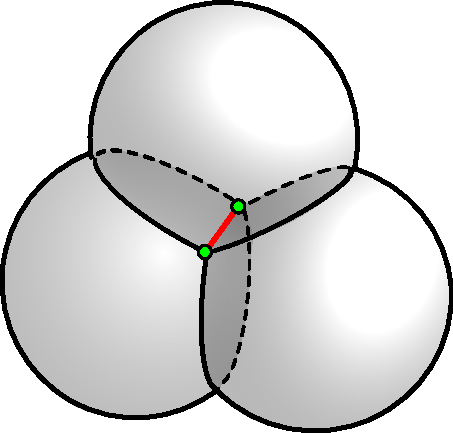
\includegraphics[width=0.3\textwidth]{Figures/3spheresIntersection.pdf}
    %\end{center}
    %\captionsetup{justification=centering}
    \caption{\normalsize Two points {(in green)} in the intersection of three spheres.}
    \label{fig:3spheres}
\end{figure}

Through this constructive procedure, once atoms \( j < i \) are fixed, atom \( i \) will have two possible positions, \( x_i \) or \( x_i^\prime \) in \( \mathbb{R}^3 \), obtained from {the} system (\ref{syst}). Once \( x_i \) is chosen from the two possibilities, we can continue the process by fixing point \( x_{i+1} \). 

A natural representation for all possible configurations \( x = (x_1,x_2,\ldots,x_n) \in \mathbb{R}^{3 \times n} \) is a binary tree, where \( x_{1},x_{2},x_{3} \) are represented as a single root node (since they are fixed) and their two children represent the two possibilities for \( x_4 \), and for each of these, the two possibilities for \( x_5 \) and so on (see Figure \ref{fig:binary_tree}). 

\begin{figure}[H]
   % \begin{center}
        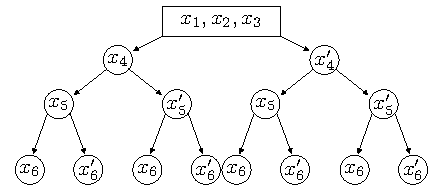
\includegraphics[width=0.6\textwidth, clip]{Figures/binary_tree.pdf}
    %\end{center}
    %\captionsetup{justification=centering}
    \caption{\normalsize Binary tree associated with a DDGP instance with six atoms.}
    \label{fig:binary_tree}
\end{figure}

If we designate the left node as child \( 0 \) and the right one as child \( 1 \), we can also map the relative position of each realization of \( x_i \) with respect to the plane \( \pi_i \) defined by \( x_{j},x_{k},x_{l} \), where \( j,k,l \) are the reference atoms of the \( i \)-th atom. Specifically, we can define the vectors $$\vec{u}=x_{j} - x_{l},\;\; \vec{v}=x_{k} - x_{l},\;\; \vec{w}=x_{i} - x_{l},$$ and assign orientation \( 0 \) if \( \vec{w}\cdot(\vec{u}\times \vec{v}) < 0 \), and \( 1 \) otherwise (see Figure \ref{fig:semispace}).

\vspace{-4pt}\begin{figure}[H]
   % \begin{center}
        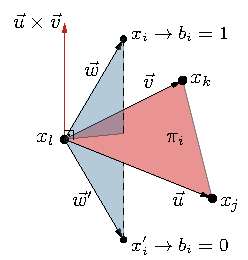
\includegraphics[width=0.4\textwidth, clip]{Figures/semispace.pdf}
    %\end{center}
    % \captionsetup{justification=centering}
    \caption{\normalsize Plane \( \pi_i \) and the positions \( x_i \) and \( x_i' \) associated with orientations \( 0 \) and \( 1 \). {Plane \( \pi_i \) is colored in light red. The perpendicular vector $\vec{u}\times \vec{v}$ is colored in red. The possible immersion points (in $\mathbb{R}^{3}$) for the vertex $v_{i}$ are $x_{i}$ and $x'_{i}$: the point ``above'' the plane $\pi_{i}$ is $x_{i}$ and has orientation $b_{i}=1$; the point ``below'' $\pi_{i}$ is $x'_{i}$ and has orientation $b_{i}=0$.}}
    \label{fig:semispace}
\end{figure}

The search for solutions within the DDGP binary tree can be attempted using brute force. However, this approach becomes impractical for molecules with {hundreds of atoms as the size} of the tree grows exponentially with the number of atoms.

When additional distances, namely \( d_{ij} \) where \( j \) is not one of the reference atoms of atom \( i \), are known, the viable configurations are reduced by the presence of the additional constraint \( \|x_i-x_j\|_2=d_{ij} \). These additional constraints are referred to as \emph{pruning constraints}, as they render branches in the DDGP binary tree infeasible. 

The BP algorithm was developed to solve the problem by intelligently {traversing} the DDGP search tree. Using the pruning constraints, it prunes branches that are identified as unfeasible, thus eliminating the need to explore the entire tree.

In its search for solutions to the DDGP, the BP algorithm explores paths in the associated binary tree using a DFS strategy that arbitrarily favors the \( 0 \) nodes of the binary tree. For example, in a binary tree of length two, the explored paths would be \( 00, \ 01, \ 10, \ 11 \).

DFS is a fundamental algorithm used in tree traversal \cite{cormen2022introduction}, characterized by exploring a branch as deeply as possible before backtracking to explore other branches. While it always finds solutions in finite trees (size dependent), DFS is notable for its memory efficiency, as it only needs to store a stack of nodes on the current path from the root node. However, it is important to note that DFS does not guarantee the shortest path to the solution.

In contrast to DFS, we propose a Best-First Search strategy, called \emph{Frequency-Based Search} (FBS), an algorithm that traverses the tree selecting which path to follow based on an evaluation function that estimates which nodes are most likely to lead to a solution.

\section{An FBS Approach Defined by the PDB}

The Protein Data Bank (PDB) is a crucial resource for scientific advancement, containing over {one} terabyte of structural data for proteins, DNA, and RNA. The archive grows by nearly 10\% per year and facilitates over 2 million structure data file downloads daily~\cite{RCSB23About}. There are 184,318 protein-related entries in the PDB, of which 14,134 were obtained through NMR \cite{RCSB23GrowthNMR}.

To assemble our data repository, we selected all protein structures derived from NMR experiments present in the PDB, considering the relevance of such a technique to the scope of our research. From {the first model of} each selected PDB file, we extracted the following information for the backbone atoms of the protein in question: its unique index, its name ($N$, $C_\alpha$, $C$, $H$, $H_\alpha$), and its coordinates in $\mathbb{R}^{3}$, as well as the index and three-letter abbreviation of the residue it belongs to.

It is important to highlight that some PDB files do not completely describe the protein backbone. For example, there are files in which some residues are missing, and in others, some atoms are missing. We also chose to remove proline and glycine residues, as these amino acids exhibit unique geometric characteristics and are often studied separately in the literature \cite{lovell2012structValidationCalpha,morris1992stereochemical,
read2011new}.

We refer to the stretches of the backbone formed by contiguous residues after the removal of prolines and glycines as \emph{protein segments}. Thus, associated with each PDB file, we generated several files, one for each protein segment. The total number of protein segments obtained from all the NMR files in the PDB is 72,983.

\subsection{An Example of a DDGP Order to Be Used in the FBS}

To establish an FBS strategy to explore the DDGP search tree, inspired by the PDB data, one must first determine a DDGP order for the atoms in the backbone. We present a DDGP ordering that groups atoms in residues {and} utilizes the length of covalent bonds and bond angles, as well as the geometric properties of peptide planes.

In the context of protein geometry, it is considered that bond lengths and bond angles {are fixed despite the natural} internal motions of proteins. This assumption is known as the \emph{rigid geometry hypothesis} \cite{gibson1997energyMinRigid}. Consequently, the distances between atoms connected by one or two covalent bonds are known. In addition to this distance information, it is well established in the biological literature that the atoms ``around'' a peptide bond belong to the same plane, implying that all distances between these atoms are also known \cite{lavor2019minNMRrigidity}. Since the peptide bond connects the carboxyl carbon of the i-th residue ($C^{i}$) to the amine nitrogen of the (i+1)-th residue ($N^{i+1}$), the atoms in the i-th peptide plane are $C_{\alpha}^{i}$, $C^{i}$, $N^{i+1}$, $C_{\alpha}^{i+1}$ (see Figure \ref{fig:peptide_3_amino_with_rho}). We also consider that the distances between $H^{i}$, $H_{\alpha}^{i}${,} and $H_{\alpha}^{i}$, $H^{i+1}$ can be detected by NMR \cite{guntert1998structBioNMRdata,rowland1996intermolecularContact,billeter1982sequentialhNMRspectra}.

Based on these properties, we use the following DDGP order for atoms in the protein backbone:
\begin{equation}\label{eq:ddgp_ordem_1}
    \rho = ( N^{1}, C_{\alpha}^{1}, H_{\alpha}^{1}, C^{1}, \, \dots \, , H^{i}, N^{i}, C_{\alpha}^{i}, H_{\alpha}^{i}, C^{i}, \, \dots \, , H^{n}, N^{n}, C_{\alpha}^{n}, H_{\alpha}^{n}, C^{n}).
\end{equation}

Figure \ref{fig:peptide_3_amino_with_rho} illustrates the ordering $\rho$ for a three-residue peptide. The numbers inside the circles indicate the index of the atoms in the ordering.

\begin{figure}[H]
    %\begin{center}
        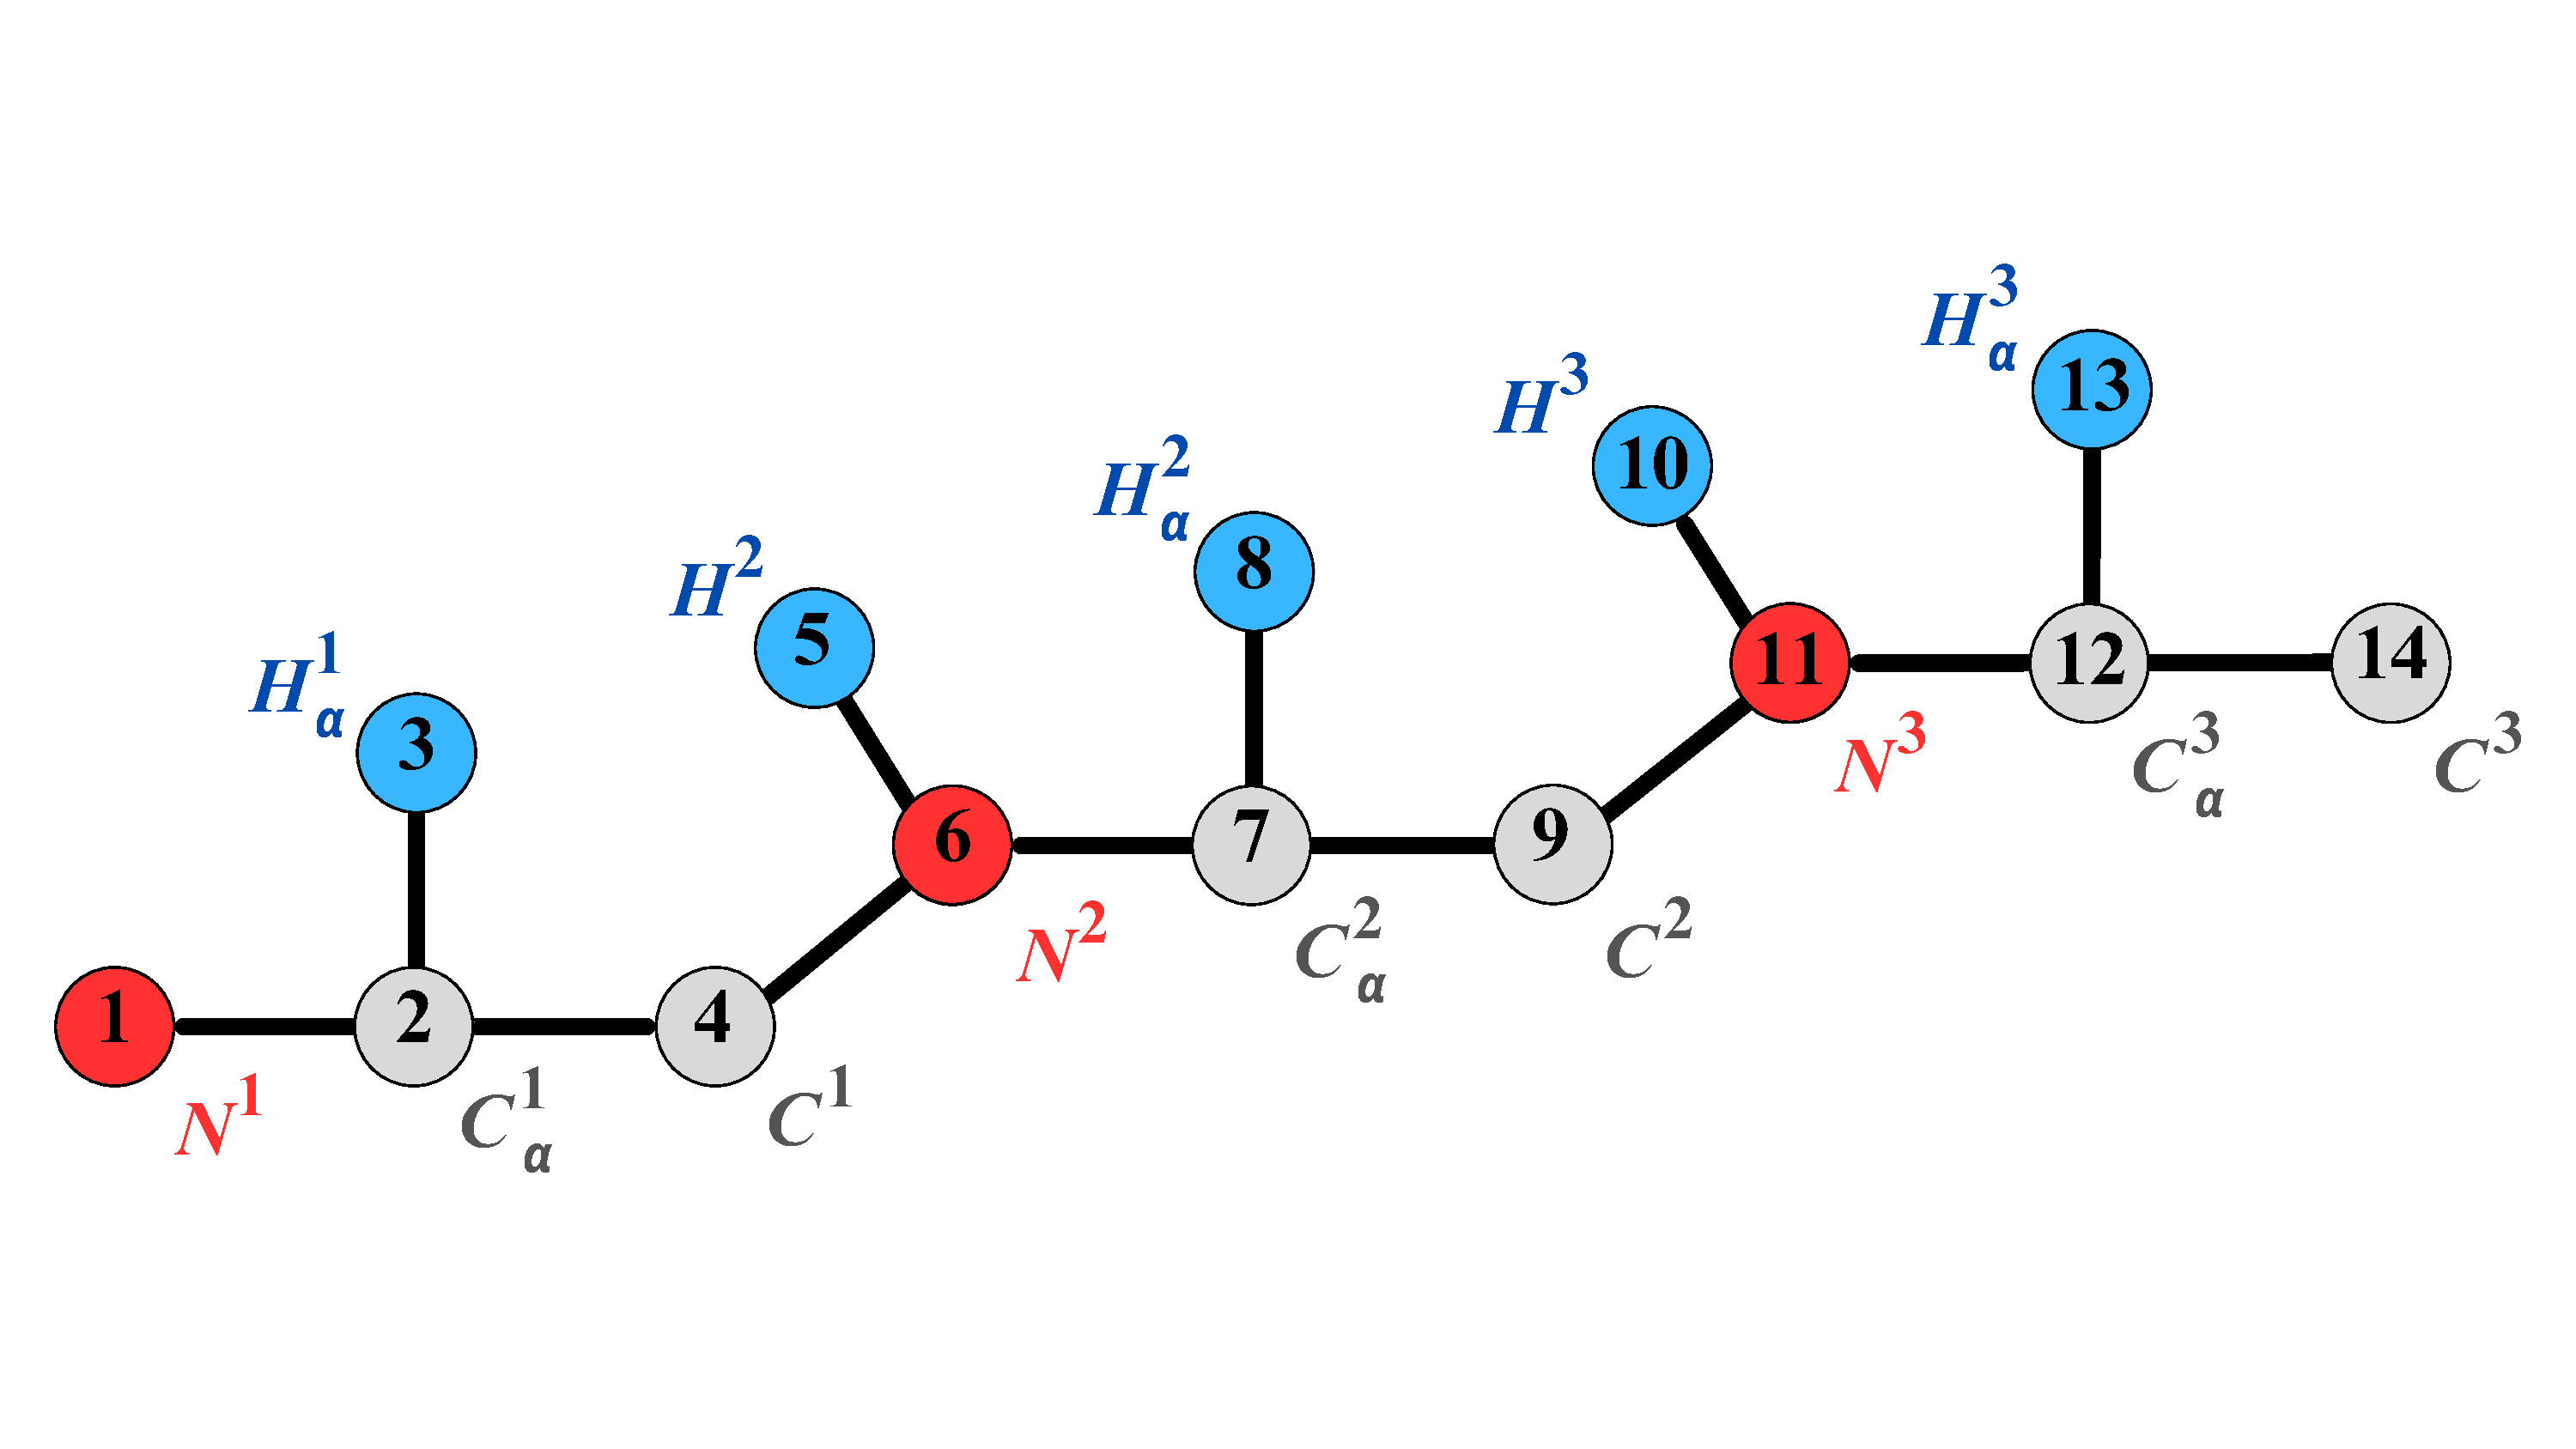
\includegraphics[width=0.8\textwidth]{Figures/peptideo3aminoacidos_comRho.pdf}
    %\end{center}
    % \captionsetup{justification=centering}
    \caption{\normalsize Order $\rho$ of a 3-residue peptide backbone. {The nitrogens are represented in red; the carbons in gray; and the hydrogens in blue. The number inside each circle represents the position of the respective atom in the order $\rho$.}}
    \label{fig:peptide_3_amino_with_rho}
\end{figure}

Table \ref{tab:predecessors_rho} shows, for each element $v$ in $\rho$, the three reference atoms of $v$, the coordinates and distances to $v$ of which are used to immerse $v$ in $\mathbb{R}^{3}$ (column ``Predecessor Atoms''), as well as their positions in $\rho$ (column ``Predecessor Positions''). Note that all the residues consist of five atoms, except for the first, which is composed of four atoms.


\begin{table}[H]
\caption{\normalsize The DDGP order related to $\rho$. {For each atom in $\rho$: first column displays its position; the second column displays its symbol; the third column displays the positions in $\rho$ of its reference atoms; the fourth column displays the symbols of its reference atoms.}}\label{tab:predecessors_rho}
\small
\centering
\begin{tabularx}{\textwidth}{lccccccc} \toprule
    \textbf{Order} & \textbf{Atom} & \multicolumn{3}{c}{\textbf{Predecessor Positions}} & \multicolumn{3}{c}{\textbf{Predecessor Atoms}} \\ \midrule
    $1$ & $N^{1}$ & & & & & \\
    $2$ & $C_{\alpha}^{1}$ & & & & & \\
    $3$ & $H_{\alpha}^{1}$ & & & & & \\
    $4$ & $C^{1}$ & $3$ & $2$ & $1$ & $H_{\alpha}^{1}$ & $C_{\alpha}^{1}$ & $N^{1}$ \\
    $\vdots$ &  &  &  & \\
    $5(i-1)$ & $H^{i}$ & $5(i-2) + 4$ & $5(i-2) + 3$ & $5(i-2) + 2$ & $C^{i-1}$ & $H_{\alpha}^{i-1}$ & $C_{\alpha}^{i-1}$ \\
    $5(i-1) + 1$ & $N^{i}$ & $5(i-1)$ & $5(i-2) + 4$ & $5(i-2) + 2$ & $H^{i}$ & $C^{i-1}$ & $C_{\alpha}^{i-1}$ \\
    $5(i-1) + 2$ & $C_{\alpha}^{i}$ & $5(i-1) + 1$ & $5(i-1)$ & $5(i-2) + 4$ & $N^{i}$ & $H^{i}$ & $C^{i-1}$ \\
    $5(i-1) + 3$ & $H_{\alpha}^{i}$ & $5(i-1) + 2$ & $5(i-1) + 1$ & $5(i-1)$ & $C_{\alpha}^{i}$ & $N^{i}$ & $H^{i}$ \\
    $5(i-1) + 4$ & $C^{i}$ & $5(i-1) + 3$ & $5(i-1) + 2$ & $5(i-1) + 1$ & $H_{\alpha}^{i}$ & $C_{\alpha}^{i}$ & $N^{i}$ \\
    $\vdots$ &  &  &  & \\
    $5(n-1)$ & $H^{n}$ & $5(n-2) + 4$ & $5(n-2) + 3$ & $5(n-2) + 2$ & $C^{n-1}$ & $H_{\alpha}^{n-1}$ & $C_{\alpha}^{n-1}$ \\
    $5(n-1) + 1$ & $N^{n}$ & $5(n-1)$ & $5(n-2) + 4$ & $5(n-2) + 2$ & $H^{n}$ & $C^{n-1}$ & $C_{\alpha}^{n-1}$ \\
    $5(n-1) + 2$ & $C_{\alpha}^{n}$ & $5(n-1) + 1$ & $5(n-1)$ & $5(n-2) + 4$ & $N^{n}$ & $H^{n}$ & $C^{n-1}$ \\
    $5(n-1) + 3$ & $H_{\alpha}^{n}$ & $5(n-1) + 2$ & $5(n-1) + 1$ & $5(n-1)$ & $C_{\alpha}^{n}$ & $N^{n}$ & $H^{n}$ \\
    $5(n-1) + 4$ & $C^{n}$ & $5(n-1) + 3$ & $5(n-1) + 2$ & $5(n-1) + 1$ & $H_{\alpha}^{n}$ & $C_{\alpha}^{n}$ & $N^{n}$ \\ \bottomrule
\end{tabularx} 
\end{table}

It should be emphasized that, for each element of $\rho$, except for the nitrogen atoms ($N^{i}$), the reference atoms are the three immediate predecessors (see Table \ref{tab:predecessors_rho}).

\subsection{Binary Representation for the Protein Backbone}

There are different representations for proteins. In principle, they can be represented by strings formed from 23 characters, each representing one of the possible amino acid residues. This is a unique representation but is not geometric.~Another possible representation is a list of three-dimensional coordinates defining the location of each atom composing the protein.

Since the solution space of a DDGP can be organized as a binary tree, a solution can be represented as a binary string that incorporates geometric information. Formally, following the ordering $\rho$ (given in (\ref{eq:ddgp_ordem_1})), each atom at position $x_i$ can be associated with a bit $b_i$ based on its relative position to the plane formed by its reference atoms (see Section \ref{sec2}). Thus, the Cartesian coordinates of each protein segment can be mapped, in a one-to-one relationship, to a \emph{binary sequence} $b=(b_1,\ldots,b_n)$.

Given that the first three atoms of $\rho$ are easily fixed in $\mathbb{R}^{3}$ and have no reference atoms (see Figure \ref{fig:peptide_3_amino_with_rho}), we consider $b_{1} = b_{2} = b_{3} = 0$, without the loss of generality. It is noted that for the fourth atom of $\rho$, the two possible positions for immersing it in $\mathbb{R}^{3}$, resulting from the intersection of the spheres associated with $x_1,x_2$ and $x_3$, are always both feasible, as $v_{4}$ never has a fourth preceding neighbor. This implies that for every solution $x$ where $b_{4} = 0$, there exists another solution $x’$, where $b_{4} = 1$, obtainable by reflecting $x$ with respect to plane $\pi_4$ that passes through points {$x_{1}$, $x_{2}$, and $x_{3}$}.

As a direct consequence of this unique characteristic of $v_{4}$, we know that the binary representation of $x'$ is the total inversion of the bits of $b$ from the fourth position onwards. Therefore, to reduce the representation of structures obtained in this manner, we normalize our dataset by inverting all binary representations where $b_{4}=1$. With this choice, the binary representations in our database have the format $b=(0,0,0,0,b_{5},\ldots,b_{n})$. We adopt the reduced representation $s=(b_5, \ldots, b_{n}) \in \{0,1\}^{n-4}$, removing the fixed bits.

\subsection{Extracting Binary Subsequences}

The known distances \emph{a priori} relate either atoms within the same residue or the atoms of consecutive residues.~In addition, it is known that small stretches of proteins can follow geometric patterns.~Particularly, Ramachandran plots highlight some of these patterns for sequences of three residues \cite{ramakrishnan1965stereochemicalCriteria}. To incorporate the geometric relations between adjacent residues, we extracted all \emph{binary subsequences} associated with groups of up to five consecutive residues in a protein chain.

It should be noted that, except for the first residue in a protein segment, each residue is composed of five distinct atoms to be considered, namely, $N$, $C_\alpha$, $C$, $H$, and $H_\alpha$, as illustrated in Figure \ref{fig:peptide_3_amino_with_rho}. Consequently, the binary subsequences obtained vary in {length} with the number of consecutive residues considered, being 5, 10, 15, 20, and 25 bits, respectively.

Each extracted subsequence is related to the four bits immediately preceding it. As only the first subsequence is guaranteed to be normalized, i.e., the bit preceding it is defined as $0$, it may be necessary to invert all bits of the analyzed subsequence to maintain the normalization of the strings in consideration. Therefore, in all cases, a check is made of the binary value of the atom immediately before the first atom of the binary subsequence in question. If this value is $1$, all binary values in the subsequence are inverted.

For example, consider a five-residue segment with the following reduced binary sequence:
\begin{equation}
s \, = \, (1, 0, 0, 1, 1, 0, 1, 1, 1, 0, 0, 0, 1, 1, 0, 1, 0, 1, 0, 1),
\end{equation}
where the complete sequence $b = (0,0,0,0,s)$ includes the bits of the first residue.

The sections of $s$ associated with each of its residues are
\begin{flalign}
\begin{aligned}
Residue \,\, 2 & : & (1, 0, 0, 1, 1 &, \phantom{)} \\
Residue \,\, 3 & : & \phantom{(} 0, 1, 1, 1, 0 & , \phantom{)} \\
Residue \,\, 4 & : & \phantom{(} 0, 0, 1, 1, 0 & , \phantom{)} \\
Residue \,\, 5 & : & \phantom{(} 1, 0, 1, 0, 1 & ).
\end{aligned}
\end{flalign}

Regarding the reduced sequence represented by $s$, we collect four subsequences from one residue, three subsequences from two residues, two subsequences from three residues, and one subsequence from four residues. Note that the sequence $s$ is composed of bits associated with only four residues, which implies the absence of subsequences containing five residues.

The binary subsequences of three consecutive residues to be collected are those associated with the residue triplets (2, 3, 4) and (3, 4, 5), with $s_1 = (1, 0, 0, 1, 1, 0, 1, 1, 1, 0, 0, 0, 1, 1, 0)$ and $s_2 = (0, 1, 1, 1, 0, 0, 0, 1, 1, 0, 1, 0, 1, 0, 1)$, respectively. The binary value at the position in $s$ immediately before the section associated with residues (3, 4, 5) is $1$ (i.e., the binary of the last position of \emph{Residue 2}).~Therefore, all binaries of $s_2$ should be inverted: $s_2 \leftarrow (1, 0, 0, 0, 1, 1, 1, 0, 0, 1, 0, 1, 0, 1, 0)$.

Our complete dataset with its 72,983 three-dimensional configurations and the respective binary codings can be automatically generated by the Python script available in the repository \url{https://github.com/romulomarques/proteinGeometryData} (accessed on 25 November 2023). In this repository, we also provide a \emph{.csv} file containing the PDB IDs of all the instances that we downloaded.

\subsection{The FBS Evaluation Function}

A solution to the DDGP is represented by a viable path from the root to a leaf in the binary tree of its solution space. In DFS, the search for such a path is performed in depth, preferring the node $0$ at each level. In the new search strategy, FBS seeks to identify a viable path based on the frequency of binary subsequences of lengths $5$, $10$, $15$, $20$, and $25$. More specifically, we group the subsequences by {length}, count the frequency of each occurrence, and order them in descending frequency within each group.

Although the DDGP tree may have a height greater than $25$, we restrict our analysis to subsequences of {lengths} $5$, $10$, $15$, $20$, and $25$ for two reasons: the first is that subsequences of lengths that are multiples of five represent residues with all five of their atoms; and the second is that the frequency of subsequences larger than $25$ is relatively low compared to the number of possible subsequences of smaller {lengths}. In situations where the DDGP tree has a height greater than the considered subsequences, the FBS strategy can be employed to incrementally construct a preferential path by concatenating consecutive subsequences.

Ideally, the optimal tree search strategy is one that requires the fewest number of visited nodes. For DFS, assuming the binary solution is $b=(b_1,\ldots,b_n)$, the number of visited nodes is given by
\begin{equation}\label{eq:custoDFS2}
DFS(b)= n + \sum_{i=0}^{n-1} b_{n-i} (2^{i+1} - 1),
\end{equation}
where $n$ is the number of nodes in the path representing the solution, and the term $b_{n-i}$ indicates whether the subtree rooted in the node to the left of the node associated with $b_{n-i}$ was visited (valued 1 in this case and 0 otherwise). When $b_{n-i}=1$, the total number of nodes in the associated subtree must be added, which is given by the factor $(2^{i+1}-1)$.

In FBS, paths associated with the most frequent sequences are tested first. Unlike DFS, FBS does not take advantage of already traveled paths. Instead, each alternative path is tested separately. Thus, if the position of $b$ in the FBS order is $k$, then $k$ paths of length $n$ must be tested, totaling a cost of
\begin{equation}\label{eq:custoFBS}
    FBS(b)=k \times n.
\end{equation}

Figure \ref{fig:nos_visitados_dfs_e_fbs} illustrates a binary tree of height four, composed of nodes numbered from 1 to 15, following the DFS visitation order. Below the tree representation, squares display the FBS ordering of the eight paths from the root to the leaves (ordering learned from the PDB). Suppose that the path $(1,9,13,14)$, highlighted in blue, is the binary representation of the solution. Also, suppose that $b$ is in the third position in the FBS order. With these assumptions, only node 15 would not be visited by DFS in the search for solution $b$, and the FBS algorithm would evaluate three paths of length four, involving a total of 12 nodes: $(1,9,10,11), (1,2,6,7),$ and $(1,9,13,14)$.

Applying Equations \eqref{eq:custoDFS2} and \eqref{eq:custoFBS}, we obtain
$$DFS(b)=4+0\times (2^{1}-1)+1\times(2^{2}-1)+1\times(2^3-1)=14$$
and 
$$FBS(b)=3\times 4= 12.$$

\begin{figure}[H]
	%\begin{center}
	    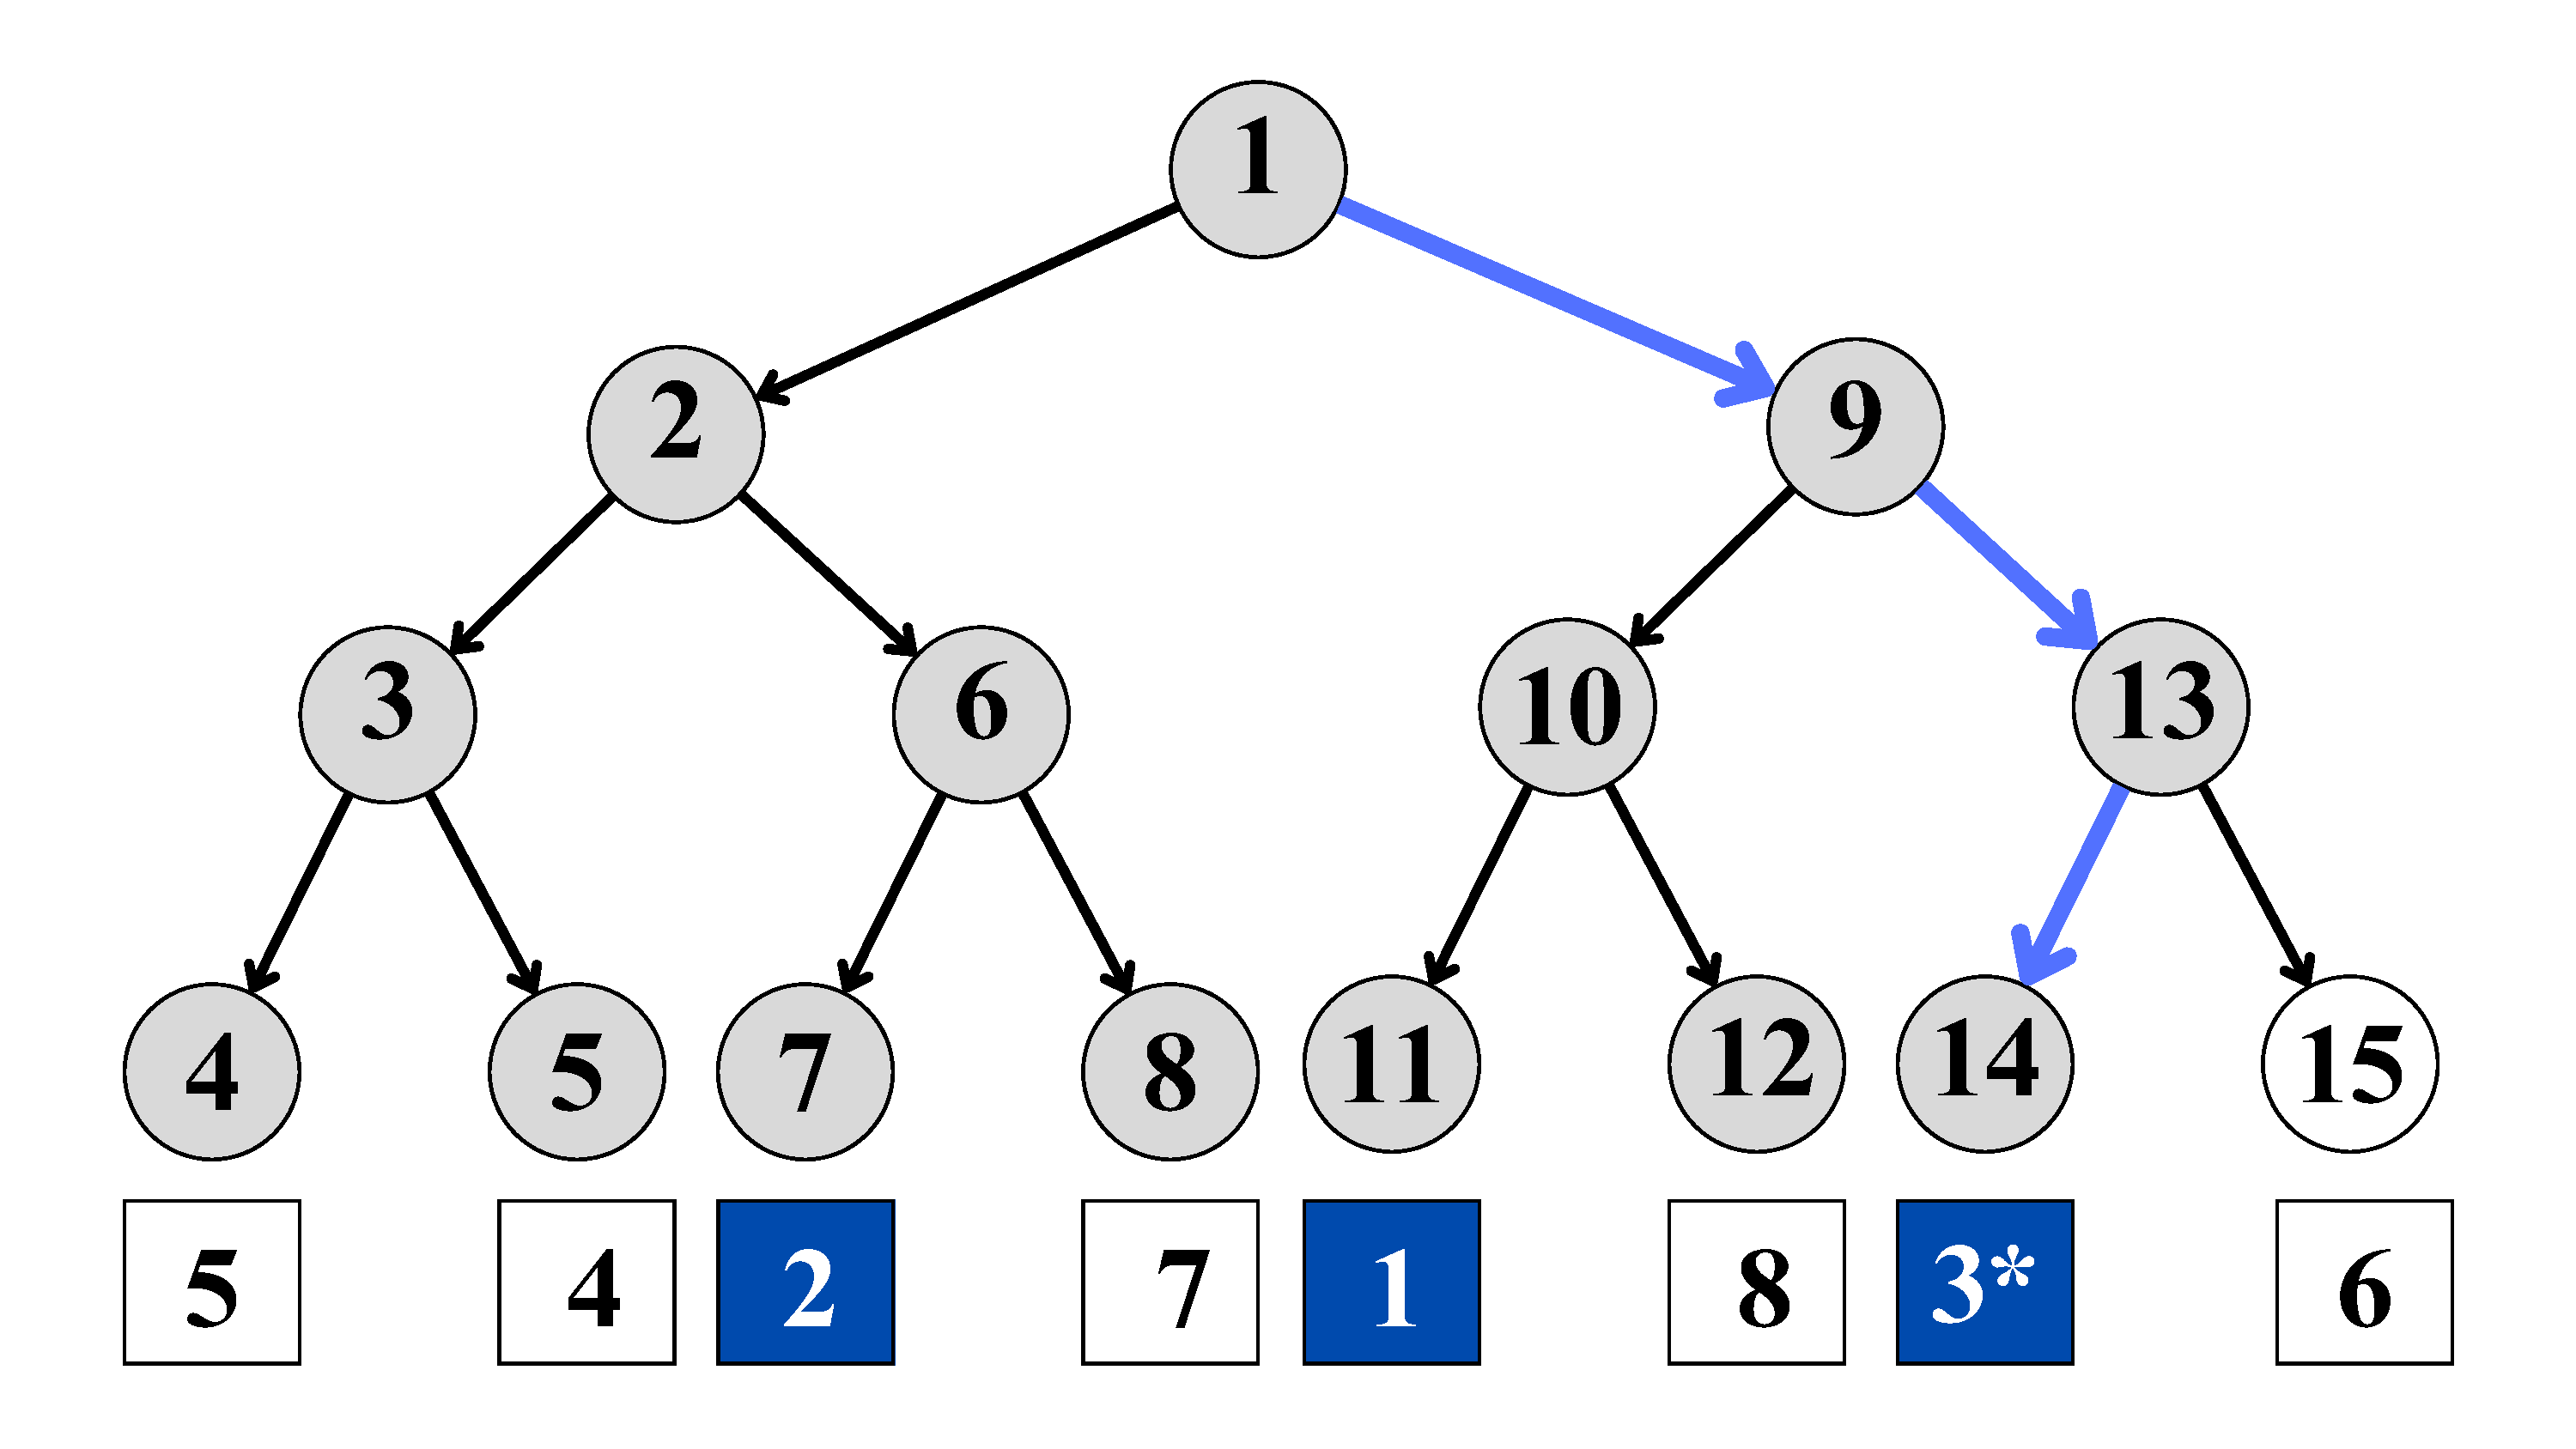
\includegraphics[width=0.7\textwidth]{Figures/nos_visitados_dfs_e_fbs.pdf}
	%\end{center}
    % \captionsetup{justification=centering}
    \caption{\normalsize Binary tree nodes visited by the DFS and FBS. The number in each node represents the node position in the visiting order of the DFS. The number in a square at the bottom of each tree leaf represents the position of the respective root--leaf path in the FBS. The arcs in blue indicate the root--leaf path corresponding to the solution of the 3-DDGP. The blue squares indicate which root--leaf paths are explored by the FBS until it finds the solution (marked with *).}\label{fig:nos_visitados_dfs_e_fbs}
\end{figure}

\section{Computational Results}

\textcolor{blue}{In this section, we present a descriptive statistical analysis of the binary subsequences processed from the segments extracted from the PDB. We highlight that the distribution of these binary subsequences is not uniform. Furthermore, we compare the performance of DFS and FBS in terms of the execution time of the SBBU algorithm.

In Table \ref{tab:unique_binary_subsequencies}, for each edge type, the column \emph{Count} denotes the number of binary subsequences present in our dataset, the column $k$ represents the number of distinct subsequences, and the column $k_{\text{max}}$ indicates the maximum number of possible binary substrings, defined as $k_{\text{max}} = 2^{length}$. The column $k/k_{\text{max}}$ reveals the fraction of observed subsequences in relation to the universe of mathematically possible subsequences. Finally, the column \emph{Count}$/k_{\text{max}}$ is the ratio of the number of binary subsequences to the maximum number of possible subsequences.

\begin{table}[H] 
\caption{\normalsize Frequency information of binary subsequences of each edge type: second column exhibits the binary subsequence lengths; third column exhibits the number of binary subsequences processed from PDB; fourth column exhibits the number of unique binary subsequences collected; fifth column exhibits the number of unique binary subsequences that are mathematically possible to exist. The sixth and seventh columns are ratios of the third and fourth columns to the fifth column, respectively.}\label{tab:unique_binary_subsequencies}
\newcolumntype{C}{>{\centering\arraybackslash}X}
\begin{tabularx}{\textwidth}{CCrrCr}
\toprule
Edge Type & $\boldsymbol{Length}$ & $\boldsymbol{Count}$ & $\boldsymbol{k}$ & $\boldsymbol{k_{max}}$ & $\boldsymbol{k/k_{max}}$ & $\boldsymbol{Count/k_{max}}$ \\
\midrule
HA\_9\_H & 7 & 78943 & 64 & 64 & 1.00 & 1233.48 \\
HA\_6\_HA & 4 & 201802 & 8 & 8 & 1.00 & 25225.25 \\
C\_4\_CA & 2 & 5826 & 2 & 2 & 1.00 & 2913.00 \\
\bottomrule
\end{tabularx}
\end{table}
}

In Table \ref{tab:unique_binary_subsequencies}, we observe that for all edge types, the fraction of observed binary subsequences ($k/k_{\text{max}}$) is equal to 1. This indicates that every possible binary subsequence of the specified length is present in our dataset. Additionally, the ratio of \emph{Count} to $k_{\text{max}}$ varies significantly across different edge types, reflecting the differing frequencies with which each subsequence occurs. For instance, the edge type HA\_6\_HA with a length of 4 has a \emph{Count}/$k_{\text{max}}$ ratio of 25,225.25, if we had a uniform distribution of subsequences, we would expect each unique subsequence to be observed 25,000 times on average. In contrast, the C\_4\_CA edge type with a length of 2 has a ratio of 2,913.00, indicating a lower average frequency per subsequence. These variations imply that while all possible binary subsequences are represented across the edge types, their occurrences are not uniformly distributed. This non-uniform distribution is a consequence of the edge ordering adopted in the SBBU.

For the application of the FBS strategy, for each edge type, we assign indices to the binary subsequences, ordering them in descending order with respect to their occurrence probabilities. In the following figures, we normalize the indices by dividing them by the total number of subsequences of each {length}. As a result, the normalized indices have values in the range $(0,1]$. That is, if we have sequences $s_1$, $s_2$, and $s_3$ with occurrence probabilities of $0.1$, $0.6$, and $0.3$, respectively, then the normalized indices would be $1/3$ for $s_2$, $2/3$ for $s_3$, and $1$ for $s_1$.

Figure \ref{fig:prune_edges_acc_prob} presents the accumulated probabilities for subsequences of each edge type, using the same normalized indices. It is observable that, edges of the type HA\_6\_HA and C\_4\_CA have a distribution close to the uniform distribution. On the other hand, the edge type HA\_9\_H has a distribution with a sharp peak at the beginning, followed by a rapid decline. So for the edge type HA\_9\_H, a small number of subsequences concentrate most of the probability mass. By giving priority to the most frequent subsequences, we can significantly reduce the computational cost to find a feasible solution to edges in HA\_9\_H class.

\begin{figure}[H]
	%\begin{center}
	    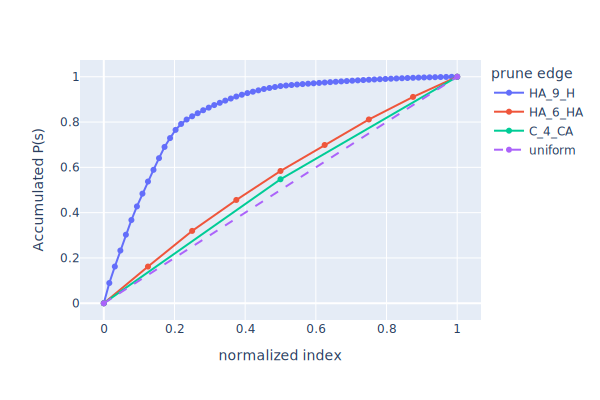
\includegraphics[scale=0.8]{Figures/prune_edges_acc_prob.svg}
	%\end{center}
    % \captionsetup{justification=centering}
\caption{\normalsize Accumulated probability of occurrence of the protein binary subsequences. Each binary subsequence configuration processed from PDB is mapped, in a descending order of probabilities, to an index in the interval $(0, 1]$.}\label{fig:prune_edges_acc_prob}
\end{figure}

In order to compare the performance of DFS and FBS, we measured the execution time of the SBBU algorithm to solve each edge, for each edge type. We also computed the execution time to solve each DMDGP instance.

Figure \ref{subfig:edge_time_speedup} shows the accumulated probability distribution for the relative time of DFS over FBS for each edge type. This relative time is called \textit{speed up}. In this context, speed up greater than 1 indicates the superior performance of the FBS algorithm compared to DFS. As can be seen, for the edge type HA\_9\_H, the FBS is better than DFS in approximately 80\% of the cases. For the edge type HA\_6\_HA, the FBS is better than DFS in approximately 60\% of the cases. And for the edge type C\_4\_CA, the FBS is worst than DFS in approximately 90\% of the cases. However, the Figure shows the average portion of the time spent by SBBU algorithm to solve each edge (constraint).  In the average, for DFS, the edge types HA\_9\_H and HA\_6\_HA correspond to about 52\% and 30\% of the total time, respectively. On the other hand, the time spent to solve the edge type C\_4\_CA is almost irrelevant. By exploring the leverage in the edge types HA\_9\_H and HA\_6\_HA and theirs relative importance in the total time, the FBS can be more efficient. Figure \ref{fig:total_edge_time_speedup} also shows that the FBS is more efficient than DFS in approximately 70\% of the cases.

\begin{figure}[H]
    %\centering
    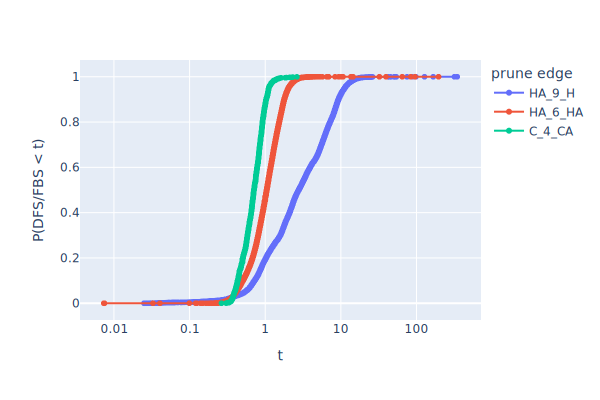
\includegraphics[width=0.8\textwidth]{Figures/edge_time_speedup.svg}
    \caption{\normalsize Ratio between the probabilities of the most frequent {(first point of a color in Figure~\ref{fig:prob_ocorrencia})} and the second most frequent {(second point of a color in Figure \ref{fig:prob_ocorrencia})} binary subsequences, for each subsequence length.}\label{fig:edge_time_speedup}
\end{figure}

\begin{figure}[H]
	%\begin{center}
	    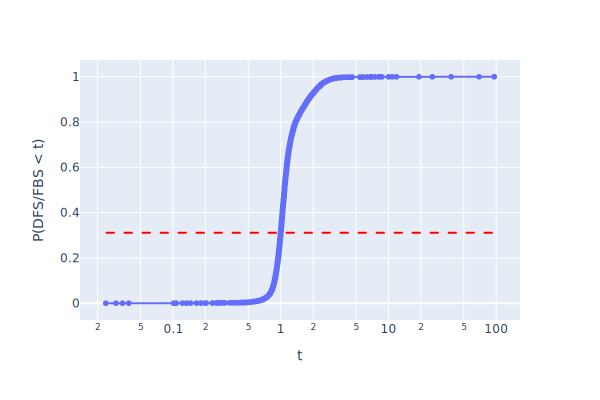
\includegraphics[scale=0.8]{Figures/total_edge_time_speedup.svg}
	%\end{center}
    % \captionsetup{justification=centering}
\caption{\normalsize Accumulated probability of occurrence of the protein binary subsequences. Each binary subsequence configuration extracted from PDB is mapped, in a descending order of probabilities, to a real index in the interval $(0, 1]$. The indexes (`x' axis) and the accumulated probabilities (`y' axis) are in logarithmic scale.}\label{fig:edge_time_speedup} also shows that the FBS is more efficient than DFS in the average.}
\end{figure}


Table \ref{tab:speedup_statistics} shows the statistics of the speed up of FBS over DFS for each edge type. It is important to note that the speed up is not a function of the edge type, but rather a property of the instance. This is because the speed up is calculated as the ratio of the cost of DFS to the cost of FBS for each instance. The mean speed up is 1.24, with a standard deviation of 1.17. The first quartile (25\%) of the speed up is 0.97, so the performance of FBS is almost equal to DFS in almost 75\% of the instances. The third quartile (75\%) of the speed up is 1.28, indicating that the performance of FBS is much better in the remaining 25\% of the instances. The distribution of the speed up is skewed to the right, with a long tail towards the higher values. This indicates that there are a few instances where FBS is much more efficient than DFS, but there are also many instances where the performance of FBS and DFS is similar.

\begin{table}[H]
    \centering
    \caption{\normalsize Statistical summary of the speed-up factor of FBS over DFS across all edge types.}
    \label{tab:speedup_statistics}
    \begin{tabular}{lr}
    \toprule
     & speed\_up \\
    \midrule
    count & 14111 \\
    mean & 1.24 \\
    std & 1.17 \\
    min & 0.02 \\
    25\% & 0.97 \\
    50\% & 1.08 \\
    75\% & 1.28 \\
    max & 95.950123 \\
    \bottomrule
    \end{tabular}
\end{table}


Figure \ref{subfig:prob_custo_rel_maior_q_alfa} displays the fraction of instances in which the cost of the DFS algorithm is at least $\alpha$ times greater than the cost of the FBS algorithm. When $\alpha=1.5$, this fraction is 50\% in instances involving the subsequences of {length} 5. However, for the subsequences of {length} 25, FBS is less costly in more than 90\% of the instances. Remarkably, for the larger instances, FBS is up to thousands of times more efficient than DFS ($\alpha=1000$). These data suggest that the performance of FBS relative to DFS increases considerably with the length of the instances.

% Second figure
\vspace{-8pt}\begin{figure}[H]
   % \centering
    \includegraphics[width=0.9\textwidth]{Figures/figF.pdf}
    \caption{\normalsize The likelihood of the relative cost (the quotient of DFS cost and FBS cost) exceeding 1.5, 10, 100, or 1000.}\label{subfig:prob_custo_rel_maior_q_alfa}
\end{figure}

{While our experiments demonstrate a discernible advantage of the FBS method over the traditional DFS, it is crucial to acknowledge a limitation in the scope of our data source. The binary subsequences that we have extracted and analyzed from the PDB represent only a specific subset of proteins, particularly those characterized using NMR techniques. Consequently, this subset may not comprehensively encompass the entire spectrum of possible protein subsequences.~This limitation is significant because the NMR subset database of the RCSB PDB might display inherent biases, reflecting only a fraction of the diverse protein structures that exist in nature.}

{Therefore, while the results indicate the promising efficiency of FBS in the context of the analyzed data, we must consider the potential impact of these biases on our findings. The dataset, primarily derived from NMR-based protein structures, might influence the frequency distribution patterns observed in our study, potentially skewing the generalizability of our results. Future research should aim to validate and extend our findings across a more diverse range of protein structures, including those determined through other methods like X-ray crystallography or cryo-electron microscopy, to ensure the broader and more unbiased application of the FBS method.}

{\color{red} In the next section, we ???}

{In summary, while our current results with the FBS method are encouraging, further investigation using a more varied dataset is essential to fully understand its applicability and limitations in the wider context of structural biochemistry.}

{\color{red}\subsection{BP algorithm with FBS}

???}

\section{Conclusions}

{This study represents a pioneering effort in integrating information from the Protein Data Bank (PDB) to solve the Discretizable Distance Geometry Problem (DDGP), a crucial model in determining protein structures via Nuclear Magnetic Resonance (NMR) data. }

{Our unique approach hinges on exploiting the combinatorial nature of the DDGP, the solution space of which is given by a binary tree. By developing a binary string representation for the coordinates of protein backbone atoms, we have observed distinctive patterns with non-uniform frequency distributions in these strings. This pivotal discovery led to the development of the Frequency Based Search (FBS) method, an innovative search technique within the DDGP solution space.}

{The efficacy of FBS over the conventional depth-first search method, as evidenced in our research, demonstrates at least 50\% more efficiency in 70\% of the cases tested. This efficiency is quantified by a reduced number of nodes visited in the search tree. Unlike the depth-first method that exhaustively explores the entire mathematical space, FBS strategically focuses on a specific subset of this space. This subset, informed by statistical data from the PDB, is more likely to yield viable and relevant solutions, thus significantly enhancing the search efficiency.}

{Expanding on the potential implications of this research, the FBS method opens up new possibilities in the realm of structural biochemistry. The efficient identification and analysis of protein structures using FBS can accelerate advancements in drug discovery, where understanding protein--ligand interactions is crucial. Additionally, this method can contribute significantly to enzyme research, aiding in the elucidation of enzyme mechanisms based on their structural configurations. In broader biochemical pathways, FBS can be instrumental in mapping out complex protein interactions, thereby providing deeper insights into cellular processes and molecular biology.}

{\color{red}

We incorporate FBS ???} into the Branch-and-Prune (BP) method represents a major advancement in computational biology. This adaptation, which effectively utilizes the geometric information available in the PDB, is set to significantly enhance the BP method's capability in protein structure determination. Consequently, our research not only marks a significant stride in computational biology but also sets the stage for transformative applications in structural biochemistry, enabling the more accurate, efficient, and comprehensive analysis of protein structures and their functions.

%%%%%%%%%%%%%%%%%%%%%%%%%%%%%%%%%%%%%%%%%%%%%%%%%%%%%%%%%%%%%%%%%%%%%
%% The "Acknowledgement" section can be given in all manuscript
%% classes.  This should be given within the "acknowledgement"
%% environment, which will make the correct section or running title.
%%%%%%%%%%%%%%%%%%%%%%%%%%%%%%%%%%%%%%%%%%%%%%%%%%%%%%%%%%%%%%%%%%%%%
\begin{acknowledgement}

{\color{red}This research was funded by Brazilian research agencies FAPESP (grant numbers 2013/07375-0 and 2023/08706-1) and
CNPq (grant number 305227/2022-0). We also extend our gratitude to the anonymous reviewers for their contributions to enhancing this paper.}

\end{acknowledgement}

%%%%%%%%%%%%%%%%%%%%%%%%%%%%%%%%%%%%%%%%%%%%%%%%%%%%%%%%%%%%%%%%%%%%%
%% The same is true for Supporting Information, which should use the
%% suppinfo environment.
%%%%%%%%%%%%%%%%%%%%%%%%%%%%%%%%%%%%%%%%%%%%%%%%%%%%%%%%%%%%%%%%%%%%%
% \begin{suppinfo}

% The Jupyter Notebook file provided by the authors at \url{https://github.com/romulomarques/proteinGeometryData} (accessed on 25 November 2023) progressively generates all files and folders used in this research. However, since some of these folders occupy a significant amount of memory, such as the folder containing the files downloaded from the PDB, which amounts to 25 Gigabytes, the authors have decided to make available in the GitHub repository the folder containing the data of protein segments, which is the necessary information to actually reproduce the experiment. In addition, in the same repository, the authors provide a \emph{.csv} file that lists the PDB IDs of all the downloaded 3D structures.

% \end{suppinfo}

\section{Data and Software Availability}

{\color{red} update here}

The Jupyter Notebook file provided by the authors at \url{https://github.com/romulomarques/proteinGeometryData} (accessed on 15 March 2024) progressively generates all files and folders used in this research. However, since some of these folders occupy a significant amount of memory, such as the folder containing the files downloaded from the PDB, which amounts to 25 Gigabytes, the authors have decided to make available in the GitHub repository the folder containing the data of protein segments, which is the necessary information to actually reproduce the experiment. In addition, in the same repository, the authors provide a \emph{.csv} file that lists the PDB IDs of all the downloaded 3D structures.


%%%%%%%%%%%%%%%%%%%%%%%%%%%%%%%%%%%%%%%%%%%%%%%%%%%%%%%%%%%%%%%%%%%%%
%% The appropriate \bibliography command should be placed here.
%% Notice that the class file automatically sets \bibliographystyle
%% and also names the section correctly.
%%%%%%%%%%%%%%%%%%%%%%%%%%%%%%%%%%%%%%%%%%%%%%%%%%%%%%%%%%%%%%%%%%%%%
\bibliography{achemso-demo}

\newpage

\section{ }

\begin{figure}[H]
        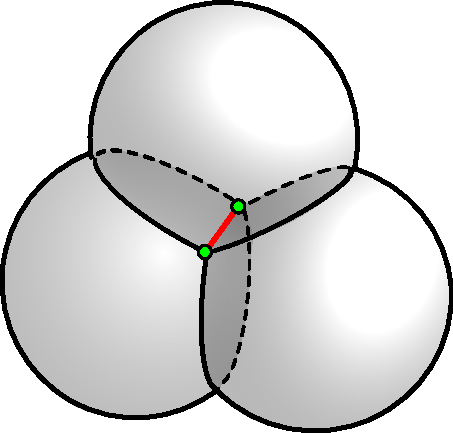
\includegraphics[width=0.3\textwidth]{Figures/3spheresIntersection.pdf}
    \caption*{\normalsize For Table of Contents Only}  
\end{figure}
\end{document}